\documentclass[Rapport]{subfiles}
\begin{document}

\section{Resultat}
\label{sec:Resultat}

% Inledande text?

I den föregående sektinonen om optimise beskrivs hur optimeringen sker.
I det här avsnittet beskrivs hur kod ser ut efter optimering och 
olika tidsjämförelser sker med och utan optimise. 
Vi testar CBN-semantiken med anropsstack.

\subsection{Raytracegrafer}

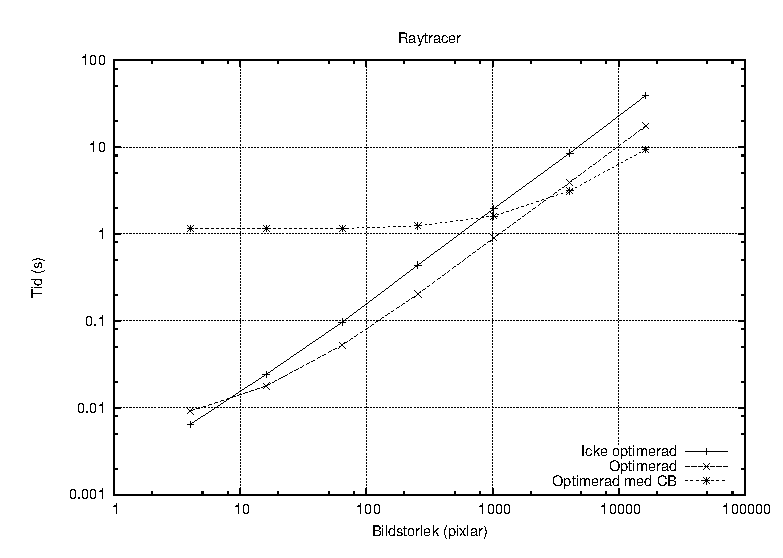
\includegraphics{shapes.eps}

\NOTE{
Den här borde ha en återkoppling till Simons genomgång om hur man använder optimise
}

\NOTE{
Shapes med och utan casebranches

Varför tar casebranches så lång tid <-> varför blir den så bra?
}

\subsection{Powergrafer}

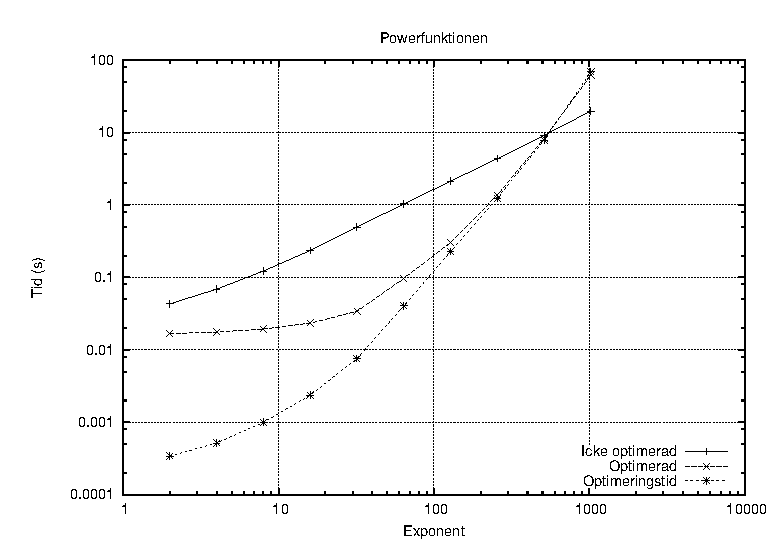
\includegraphics{power.eps}

\subsection{småexempel på mer man kan göra (med optimise)} 

Här följer några mindre exempel på vad resultatet av optimise blir:

\begin{itemize}
\item Funktionen \ic{foo} i följande exempel blir när den har applicerats på \ic{x}
en funktion som tar ett argument, \ic{y}, och adderar eller subtraherar 1 från
det beroende på värdet på \ic{x}.

\begin{codeEx}
foo x y = case x > 0 of
    { True  -> y + 1
    ; False -> y - 1
    };
\end{codeEx}
Om vi vill köra den funktionen med samma \ic{x}-värde många gånger kan den optimeras
med hjälp av \ic{optimise}, exempelvis såhär:
\begin{codeEx}
main = map (optimise (foo getInt)) getIntList;
\end{codeEx}
Om \ic{getInt} är 1 väljer optimeringsfunktionen grenen \ic{True} i \ic{case}-satsen:
\begin{codeEx}
optimise (foo 1) === \y . y + 1
\end{codeEx}

\item På liknande sätt som ovan kan funktioner som är rekursiva i ett argument
vecklas ut. Följande funktion adderar två tal steg för steg och kan vecklas ut
vid optimering:

\begin{codeEx}
add x y = case x > 0 of
    { True  -> foo (x - 1) (y + 1)
    ; False -> y
    };
\end{codeEx}

Vid optimerig av \ic{foo 2} fås följande funktion, där \ic{case}-satserna och 
rekursiva anrop har plockats bort eftersom värdet på \ic{x} är känt när
optimeringen körs:

\begin{codeEx}
optimise (add 2) === \y . y + 1 + 1
\end{codeEx}

\item ... Kända funktioner och sånt.

\end{itemize}

\subsection{vad fungerar bra och vad fungerar inte så bra allmänt (kanske flytta/merga med diskussion?)}
Optimise är bra på:
    * inlining av funktioner och primitiver
    * optimera casebranches
    * beräkna konstantuttryck i en pap och klistra in resultatet
             ( detta kan också lösas med full laziness i vissa fall - (vilka?))




\NOTE{ 

\begin{itemize}
    \item Jämför hur kod ser ut före och efter optimering. Förklara lite vad som har gjorts.
        \begin{itemize}
            \item Power har använts som löpande exempel, så vi skulle kunna visa det
                  här också.
            \item Andra program. Förslagsvis något av de lite större exempelprogrammen om vi
                   får dem att fungera bra och kan presentera det på ett vettigt sätt.
                    Shapes, regexp
        \end{itemize}
    \item Jämför snabbheten hos program med och utan optimering (benchmarks)
        \begin{itemize}
            \item Med och utan callstack för att visa hur mycket snabbare resultat det gav oss?
            \item scatterplot för en större mängd program (el. körningar)
    \item Tester med olika stora indata,
        tex listlängd pa x-axeln,
            procentuell ökning på y-axeln,
            upphöjttill-inten på z-axeln.
        
    Antagligen tillräckligt  intressant att ha 2 st av dem, tex optfunktionens storlek mot tid
                                      samt inputens storlek mot tid.
        \end{itemize}
    \item Jämför kodstorlek, komplexitet hos optimise
    \item Hur stor del av tiden går åt till att köra optimise? En graf skulle kunna visa
      detta på ena axeln och listlängd på andra axeln, för att illustrera att
      en optimerad funktion måste köras många gånger för att man ska vinna något på det.

                                      


\end{itemize}

}


\end{document}

